\chapter{基于混合纠删码的容错存储原型系统设计与实现}
为了验证预先修复技术和混合纠删码修复技术在实际应用中的性能,本章设计并实现了一个容错存储原型系统。该系统有三个特点:
(1)基于开源分布式存储中心的离散事件模拟器SimEDC进行设计实现;(2)含有丰富的混合纠删码方案,包括已有的HACFS\cite{xia2015tale}
、EC-Fusion\cite{qiu2020ec}以及LRC\&HH\cite{wang2020adaptive},支持相应的
扩展接口;(3)支持修复调度中的重建与迁移的融合。本章主在原型系统中对存储的可靠性进行分析,对不同的混合纠删码方案进行可靠行测试。

\section{系统设计}
容错存储原型系统设计主要包含以下模块:存储中心架构,节点故障模型,混合纠删码策略,节点放置策略,可靠性度量指标,事件处理模式。
\begin{figure}[H]
	\centering
	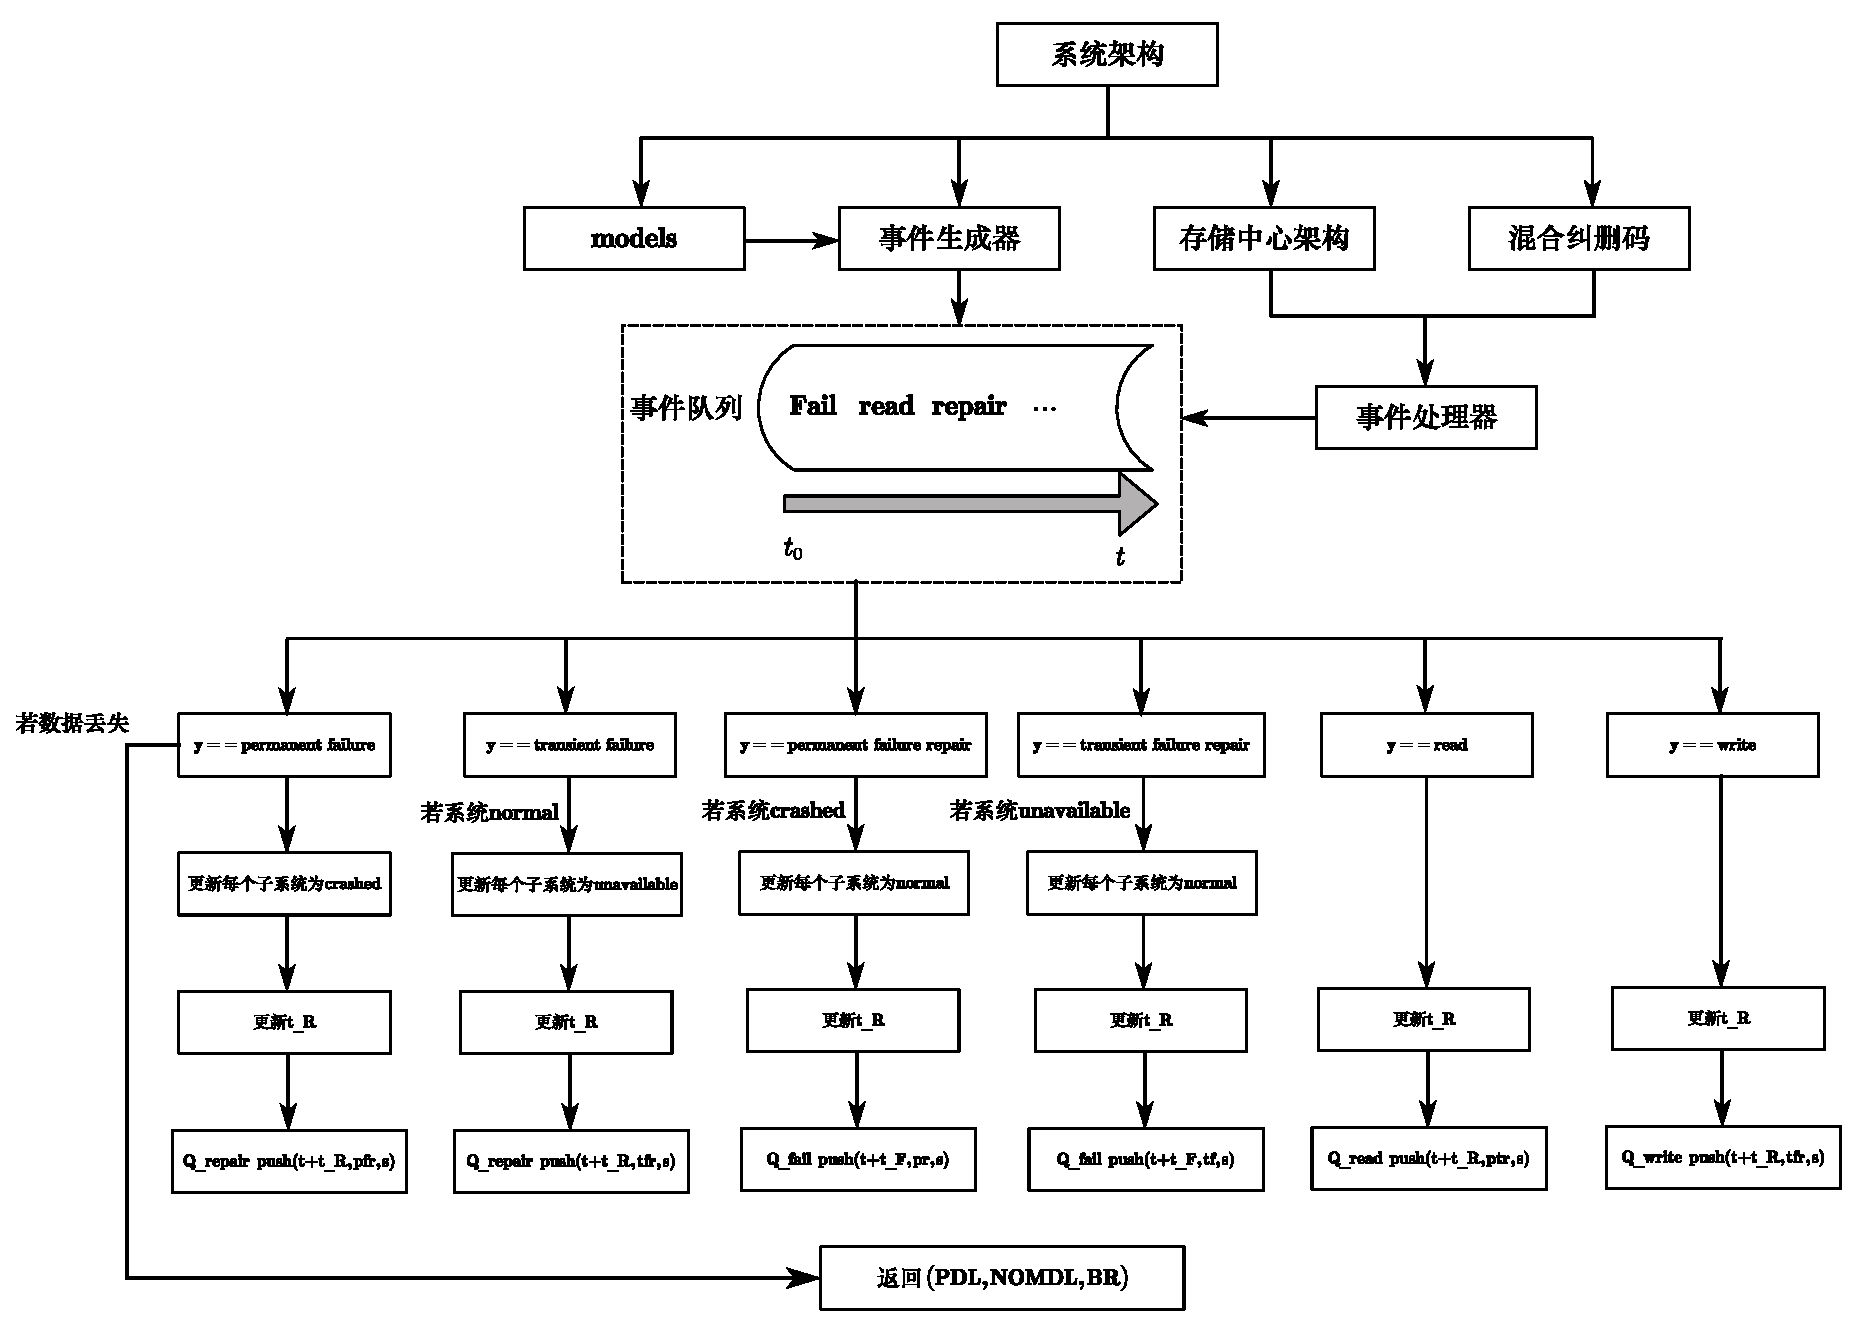
\includegraphics [scale=0.45]{figures/5.1.pdf}
	\caption{原型系统架构}
	\label{fig:5-3}
\end{figure}



\subsection{存储中心架构}
\label{sub:5.1.1}

常见的存储中心采用分层的架构来进行数据的存储和流转,
如图~\ref{fig:5-1}所示,它由多个数据柜(Rack)组成,每个数据柜上都运行着一定量的数据节点(Node)。 
每个节点连接着一个或多个磁盘,提供相应的存储空间进行数据服务。 
同一个数据柜的节点由数据交换机(ToR Switch)互联,而数据柜则由网络中心互联,
整个存储中心由各层汇聚以及交换机组成。 传统的存储中心的数据传输速度受制于数据柜之间的可用带宽,
常常达不到理论上带宽最大值,并且网络中心经常需要同时进行计算与转发操作,故性能也会受到制约。 
每个节点可以连接多个磁盘,所以虽然磁盘本身有I/O限制,依然可以实现比单个带宽更高的并行速度,
目前有两种架构形式可以缓解这种跨数据柜传输数据的带宽受限问题,分别为水平放置和层次放置。
\begin{figure}[tb!]
	\centering
	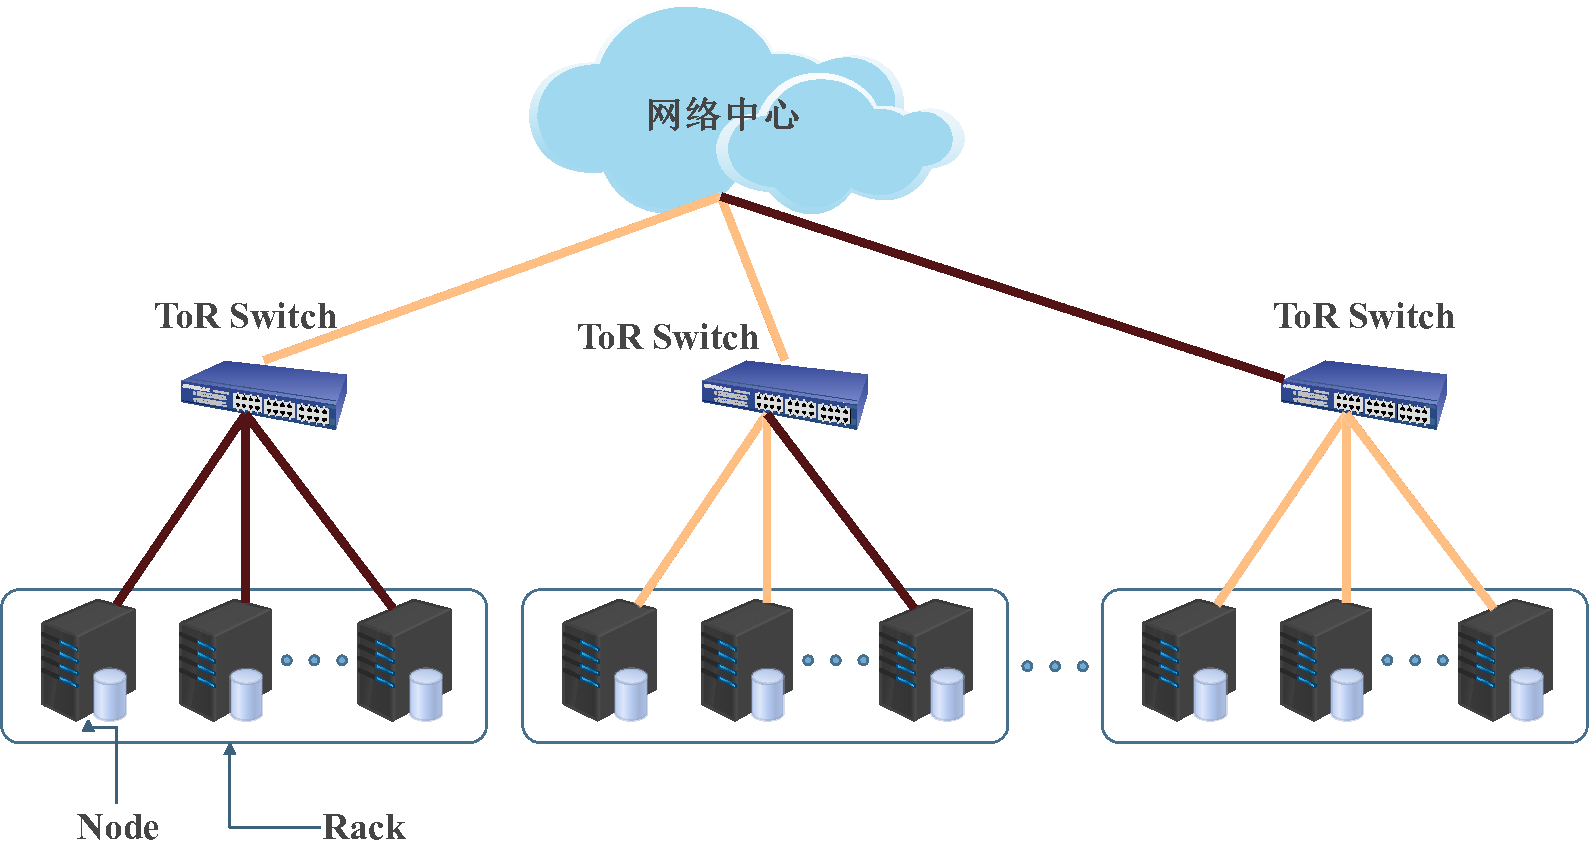
\includegraphics [scale=0.4]{figures/5-1.pdf}
	\caption{基于纠删码构建的存储系统架构}
	\label{fig:5-1}
\end{figure}

为了从多角度模拟一个存储系统的运行可靠性,将纠删码每个条带的块放置在不同的节点和数据柜中,并且为每个有$n$块的条带考虑两种放置方案:
\begin{enumerate}
    \item 水平放置:一个条带的$n$个数据块被存储在$n$个不同的节点上,
            也就是说这些节点位于$n$个不同的数据柜上(即每个数据柜上有一个块)。 
            这样的放置方式最大化地利用了节点和数据柜的容错能力。在这种情况下,
            修复一个丢失的数据块必须从其他数据柜搜索可用的数据块,从而产生了大量的跨机柜的修复传输流量,水平放置通常用于各种存储数据中心。
    \item 分层放置:一个条带的$n$个块被存储在$n$个不同的节点中,这些节点位于$r(r<n)$个数据柜中,每个节点有$\frac{n}{r}$个块,
            这里假设$n$能被$r$整除。 
            这样的放置方式减少了跨机柜之间的修复数据传输量,因为在修复任意丢失的数据块时,可以利用同一机柜中的可用块。
            相比之下,其可以容忍的机柜故障的能力比水平放置的方式要低得多。
\end{enumerate}

以RS$(6, 3)$码对水平和分层放置方式的特点进行阐述,即$n=6$, $k=3$,
将原数据文件分割成3块,并且再进行编码另外的3块,只需要其中任意3块即可恢复出原始的数据。
具体如图~\ref{fig:5-2}所示,假设一个节点想要修复其本地存储中的一个故障磁盘中的数据块,在水平放置的方式中,
一个条带的六个块都被放置在一个不同的数据柜中,所以修复丢失的数据块将从另外三个数据柜中进行块搜索。 
另一方面,在分层放置中,可以在一个数据柜中放置两个块,修复丢失的数据块可以从同一数据柜中搜索一个数据块,
再从其他数据柜中接收两个数据块,因此跨机柜的修复流量减少到两个数据块。可见分层放置比水平放置产生的跨机柜的修复流量更少。
\begin{figure}[htbp]
	\centering
	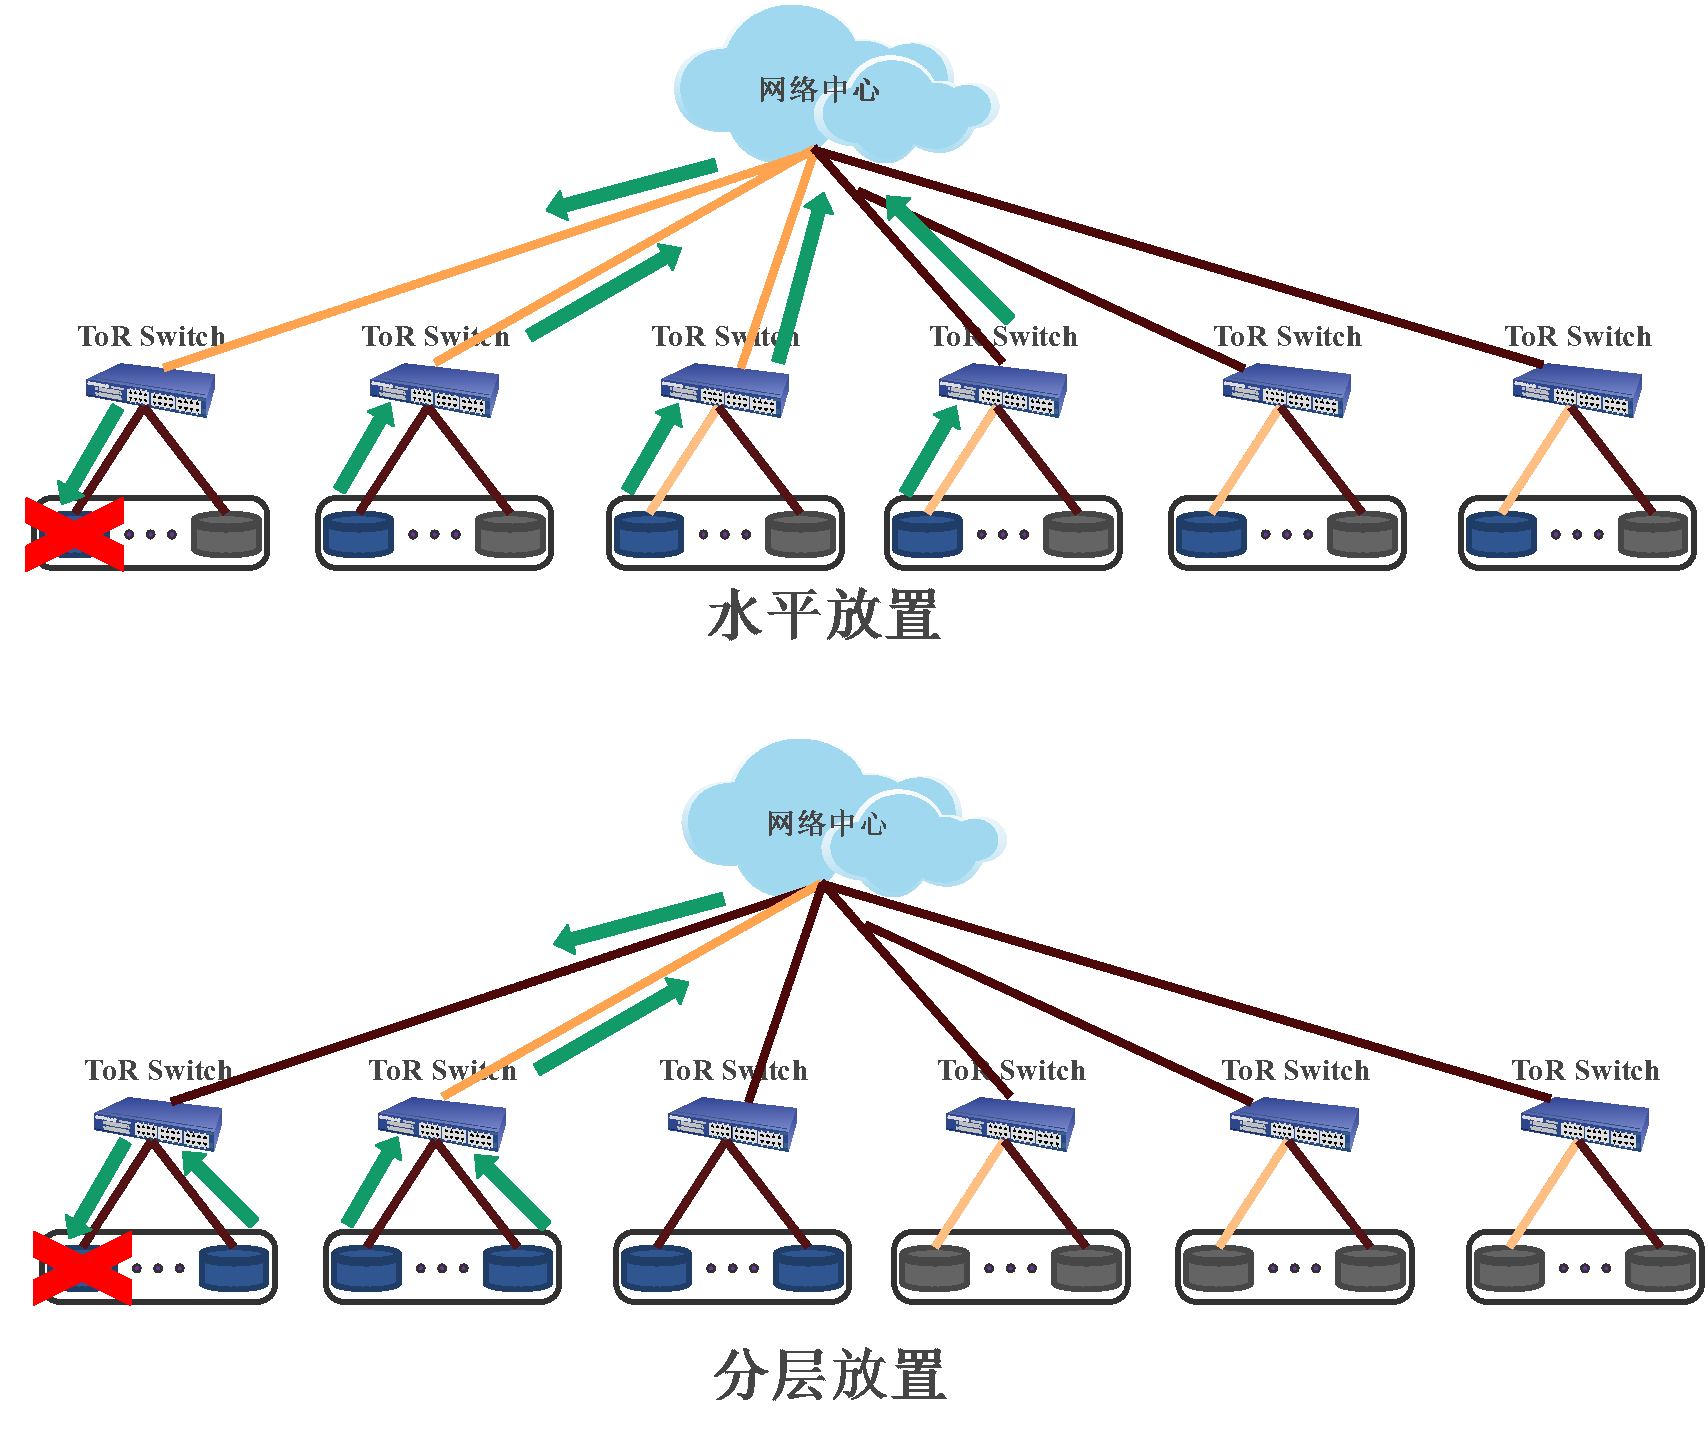
\includegraphics [scale=0.3]{figures/5-2.pdf}
	\caption{RS$(6,3)$的水平放置和层次放置}
	\label{fig:5-2}
\end{figure}

\subsection{故障模式建模}

分布式存储系统在运行中发生故障事件的概率很高,本文专注于发生在三个层面的子系统故障:
数据柜、节点和磁盘。故障本身可以是暂时性的,即一个子系统只是暂时不可用或者不可访问而不会造成实际的数据丢失
(比如网络断开、系统重启或维护),也可以是永久性的,亦即一个子系统的故障会导致永久性的数据丢失(比如磁盘损坏)。
故障可以进一步分类为是否独立,即子系统自身故障,或者关联故障,例如一些子系统由于一个共同的故障问题而发生同时故障。
关联故障往往比独立故障要严重得多,例如当一个数据柜的交换机损坏时,那么机柜内的所有节点将
失效,从而造成数据丢失。一般比较常见的故障原因是停电,在这种情况下,相当一部分节点(高达1\%)将在通电重启后损坏,并导致永久性数据丢失。 
本文采用在分布式存储系统中比较常见的四种故障模式进行模拟:

\begin{enumerate}
    \item 磁盘故障:本文专注于永久性的磁盘故障,在这种情况下,故障磁盘上的所有数据都会丢失。 为了简单起见,不考虑只破坏磁盘部分数据的潜伏扇区错误,默认一旦损坏则整个磁盘数据丢失。
    \item 节点故障:考虑暂时性和永久性的节点故障。对于前者,故障节点下的所有磁盘只是暂时不可用而没有造成数据丢失,对于后者,假设存储在该节点下的所有磁盘上的数据都全部且永久性的丢失。 
    \item 机柜故障:考虑短暂的数据柜故障,在这种情况下,故障机柜内的所有节点的数据变得无法访问,但没有产生数据丢失。
    \item 关联故障:对于发生故障的数据柜,将存储在其下的所有节点都视为故障节点,也就是关联故障会使一个机柜内的所有节点瘫痪。本文专注于永久性的关联故障,例如故障节点会发生数据不可用,类似断电现象。
\end{enumerate}

\subsection{纠删码混合策略}
\label{subsection:5.1.3}
目前比较成熟和前沿的混合纠删码技术一般是含有两种纠删码,
并对冷数据和热数据进行优化存储。其中的技术包含了在两种纠删码进行高效切换的算法,
在数据读取和写入过程中进行两种数据存储方式的转换,此外还有采取优先级队列的方式来区别冷热数据并且配以相应的纠删码方案。
一般包含三个主要特征:code选择的调整,适应性规则和code的切换。
混合纠删码策略都对于冷热数据进行了相应的划分,并且用不同的纠删码对其进行存储上传和下载。
所以在存储原型系统中需要构造相应的冷热数据划分算法,记录数据访问发生失败时的时间和节点位置,
利用这些信息可以使用LRU算法来为冷热数据划分定制自适应算法。
这里根据章节~\ref{Section:4.3}对于算法~\ref{alg:4-1}论述,为了将算法适应范围扩大,从而得到了算法~\ref{alg:5-1}。

\begin{algorithm}[htpb]
	\begin{algorithmic}[1]
		% \newlength{\commentindent}
		\setlength{\commentindent}{.3\textwidth}
		\setlength{\algorithmicindent}{1.5em}
		\renewcommand{\algorithmiccomment}[1]{\unskip\hfill\makebox[\commentindent][l]{$\rhd$~#1}\par}
		\LetLtxMacro{\oldalgorithmic}{\algorithmic}
		\renewcommand{\algorithmic}[1][0]{
			\oldalgorithmic[#1]
			\renewcommand{\ALC@com}[1]{
				\IFnum\pdfstrcmp{##1}{default}=0\ELSE\algorithmiccomment{##1}\fi}%
		}
		\REQUIRE{Queue1,Queue2 and $\eta$}
		% \ENSURE{$\textbf{NewW}$}
        \FOR{\text{Queue2头的每个插入请求}}
        \IF{flag $\neq $ Fast Code and (writes/recoveries) $< \eta$}
        \STATE set flag = Fast Code;
        \STATE convert to Fast Code;
        \ENDIF
        \ENDFOR
        \FOR{\text{Queue1头的每个插入请求}}
        \IF{flag $\neq $ Compact Code and (writes/recoveries) $\geqslant  \eta$}
        \STATE set flag = Compact Code;
        \STATE convert to Compact Code;
        \ENDIF
        \ENDFOR
        \FOR{\text{Queue2尾的每个弹出请求}}
        \IF{flag == Fast Code }
        \STATE set flag = Compact Code;
        \STATE convert back to Compact Code;
        \ENDIF
        \ENDFOR
	\end{algorithmic}
	\caption{容错存储原型系统动态自适应划分算法}
	\label{alg:5-1}
\end{algorithm}


% \subsubsection{HACFS}
% \subsubsection{EC-Fusion}
% \subsubsection{LRC和HH码}
\subsection{纠删码接口}
原型系统中的纠删码模块为数据编码提供了四个主要接口:编码(encode)、解码(decode)、编码上载(upcode)和编码下传(downcode)。 
编码操作的输入是一个原数据文件(data file)和编码方案(codec)作为输入,并为原数据文件中的分割块生成一个奇偶校验块(parity file)。 
解码操作是在块丢失后的退化读取中调用的,或者作为磁盘或节点故障时启动重建工作的一部分。 它还需要文件中丢失或损坏的块的索引(lost block index),
并使用输入的编码方案从条带中剩余的数据和奇偶块中重建丢失的块。

自适应编码模块通过调用编码上载和编码下传的操作,来进行两种编码的切换。 
这两种转换操作在改变数据文件的编码方案时只更新相关的奇偶校验文件。 
编码上载操作将数据从Fast Code转换为Compact Code,从而减少了奇偶校验文件的大小,
达到降低存储开销的目的,此外它不需要读取数据文件。 编码下传操作将数据从Compact Code转换为Fast Code表示,
从而降低修复成本,它需要读取原数据文件和奇偶性校验块,具体如表~\ref{table:5-1}所示。 

\begin{table}[htbp]
	% \setlength{\tabcolsep}{2.9pt}
    \newcommand{\tabincell}[2]{\begin{tabular}{@{}#1@{}}#2\end{tabular}} %放在导言区
	\centering
	\caption{容错存储原型系统纠删码操作接口}
	\begin{tabular}{cll}
		\toprule
        接口操作  & 输入 & 输出 \\[1pt]
		% \midrule
		\\[-15pt]
        \multirow{3}{*}{\tabincell{c}{encode \\ decode}} & data file, codec; & parity file \\
                                    & data file, parity file &  \\
                                    & codec, lost block index & recovered block \\
        \hline
        \\[-15pt]                         
        \multirow{4}{*}{\tabincell{c}{upcode \\ downcode}} 
        & parity file, original fast codec & parity file encoded with compact codec \\
        & new compact codec; & \\
        & data file, parity file & parity file encoded with fast codec\\
        & original compact codec, new fast codec & \\
		\midrule
	\end{tabular}
	\label{table:5-1}
\end{table}



\subsection{可靠性分析指标}
本文采用的是广泛运用于评估系统可靠性的度量指标,
包括数据丢失率PDL(Probability of data loss),
归一化数据损失度NOMDL(Normalized magnitude of data loss)以及
阻塞率BR(Blocked ratio)。

PDL衡量了一个存储中心在一定时间内发生任意数据块不可恢复的失效事件的
可能性(即纠删码条带中永久失效的块的数量超过了可容忍的限制),一般计算方法为失效块占总数据块的比例。

NOMDL它是由Greenan\cite{greenan2009reliability}等提出的,用来衡量预估的数据丢失量(以字节为单位)
与存储容量进行正则化。它所具有的几个关键属性改进了现有的可靠性指标,具体计算方法如公式~\ref{eq:5-1}。
\begin{equation}
	\label{eq:5-1}
	NOMDL=\frac{avg\_num\_lost\_chunks}{num\_strips\ \times \,\,code\_n}
\end{equation}


BR衡量的是由于存储一个数据块的子系统的短暂或永久的故障而不能直接访问该块的时间比例。
但是这样一个无法访问的块可能仍然可以从其他子系统中同一条带的其他可用块中恢复,
但会产生重建该块的额外开销。因此,BR的值可以代表在正常模式下(即没有故障)无法直接访问一个块的时间,
具体计算方法如公式~\ref{eq:5-2}。
\begin{equation}
	\label{eq:5-2}
	BR=\frac{sum\_unavail\_time}{num\_chunks\ \times \,\,mission\_time}
\end{equation}

\subsection{事件处理}
原型系统中的每个故障事件或修复事件都用一个由三个字段组成的元组来表示。 
(1)事件发生时的时间戳time $t$(2)事件类型type $y$(3)与事件相关的子系统subsystem $s$。
原型系统会将所有的事件存储在一个事件队列中,事件的发生机制遵从于统计模型概率表(见表~\ref{table:5-2}),
该队列以优先级队列的方式进行实现,并且返回具有最小时间戳(亦即最新发生)的事件,
供事件处理程序进行相应处理。 原型系统将分别处理永久性故障和瞬时性故障,这里考虑四种事件类型:
(1)永久性故障,(2)瞬时性故障,(3)永久性故障修复,以及(4)瞬时性故障修复。 

故障处理。 在模拟过程中,每个子系统(即机柜、节点和磁盘)都与三种状态之一有关。 
(1)正常(即没有发生故障)(2)不可用(即发生瞬时故障)和(3)崩溃(即发生永久性故障)。 
就严重程度而言,正常是最不严重的,不可用处于前后者中间状态,而崩溃是最严重的。 
假设如果一个子系统发生故障,只有当状态变得更加严重时,其状态才会被更新。 
也就是说一个正常或不可用的状态在永久性故障中会变成崩溃状态,
或者一个正常的状态在暂时性故障中会变成不可用状态。 而崩溃的状态会依旧保持不变,
同时在一个分层的分布式存储中心里,它所有的连接上它的子系统将继承同样的状态,
如果一个节点崩溃了,那么附着在该节点上的所有磁盘也会崩溃;如果一个机架(即节点)不可用,
那么该机架内的所有节点和磁盘(即所有附着的磁盘)如果原本是正常的,也将变成不可用。 

原型系统的整个运行流程就是在不断地处理来自事件队列的事件作业。 
在收到一个永久性的故障事件后,它检查存储在该子系统中的每一个块是
否可以被足够数量的同一条带的可用块修复。 如果不行,它就得出结论认为数据丢失,
并返回当前迭代的可靠性指标。 如果没有数据丢失或收到一个瞬时故障事件,
原型系统为故障子系统触发一个相同类型(即永久或瞬时)的修复事件,
并将该事件插入到事件队列中,供以后修复处理。

修复处理。 在将修复事件插入事件队列之前,原型系统计算出修复永久性或暂时性故障所需的修复时间。 
对于永久性故障,修复时间的计算方法是将所有故障块的跨机柜修复流量总量除以可用的跨机柜带宽。 
对于瞬时故障,修复时间由统计模型或相应子系统的事件追踪来决定。

读取和写入。 当读取和写入事件发生时,将根据算法~\ref{alg:5-1}的方法进行纠删码的决策并且计算出修复和读取时间。 
对于读取首先判断节点是否处于故障状态,然后再进行读取时间和纠删码切换的时间计算,
对于写入同理,区别在于不需要切换,需要计算跨柜放置节点数据的传输流量。 

当从事件队列中收到一个修复事件时,
原型系统将相关子系统的状态更新为正常状态。 
此外,如果任何子系统有相同的故障类型,
同时也会将其状态更新为正常状态。 
例如,如果一个崩溃(标记为unavailable)的节点被修复,
则与其相关的任何一个崩溃的磁盘也被修复,其状态变成正常。 
最后,原型系统为子系统创建下一个相同类型(即永久或短暂)的故障事件,
并将该事件插入到事件队列中,以便以后处理故障。

本文采用的的默认故障和修复事件统计模型概率表的如表~\ref{table:5-2}所示. 其中$W=(\beta,\eta,\gamma)$表示
Weibull分布且带有形状参数$\beta$,尺度参数$\eta$,位置参数$\gamma$。$EXP(\lambda)$表示带有
参数$\lambda$的指数分布。


\begin{table}[htbp]
	% \setlength{\tabcolsep}{2.9pt}
    % \newcommand{\tabincell}[2]{\begin{tabular}{@{}#1@{}}#2\end{tabular}} %放在导言区
	\centering
	\caption{默认故障和修复事件统计模型表}
	\begin{tabular}{lll}
		\toprule
        故障类型  & 故障时间 & 修复时间 \\[1pt]
		% \midrule
        \hline
        \\[-15pt]  
        Permanent disk failures & $W(1.12, 10 years, 0)$ & $\frac{cross-rack\,\,repair\,\,traffic}{cross-rack\,\,bandwitdth}$ \\
        Permanent node failures & $EXP\left( \frac{1}{125 months} \right) $ &  \\
        Transient node failures & $EXP\left( \frac{1}{4 months} \right) $ & $EXP\left( \frac{1}{0.25 hours} \right) $ \\
        Transient rack failures & $EXP\left( \frac{1}{10 years} \right) $ & $W(1, 24 hours, 10)$ \\
        Permanent correlated failures & $EXP\left( \frac{1}{1 year} \right) $ & $EXP\left( \frac{1}{15 hours} \right) $ \\
		\midrule
	\end{tabular}
	\label{table:5-2}
\end{table}





\section{实验结果与分析}
\subsection{实验设置}
系统基于Python3实现并进行数据运行测试,测试平台操作系统为Ubuntu 16.04 LTS,
配置为3.70GHz Intel Core i5-9600K处理器,16GB内存,1 Gbit/s网络接口。

实验中的主要输入参数详情包括,place\_type接收两种参数的输入:flat和hie,
基于节~\ref{sub:5.1.1}
提到的节点放置策略进行实现;code\_type参数接收三种输入,分别为hacfs(HACFS),ecf(EC-Fusion),
lrchh(LRC\&HH),基于节~\ref{subsection:5.1.3}中论述的三种混合纠删码策略进行实现。
实验中为了便于方便分析不同纠删码策略的可靠性数据,
针对混合策略的参数输入保持不变,其他单一纠删码实验的参数进行改变进行对比实验。
具体为cross-rack bandwidth设置为1Gb/s,place\_type设置为flat,chunk\_size设置为64MB等。 

\subsection{PDL参数实验结果}
如图~\ref{fig:5-4}所示是PDL多次实验的结果,误差区间是$\pm 4\%$。
误差是通过实验得到的数据结果的范围进行确定的,
不同的方案的结果范围不尽相同,
同时也可以确定其在真实运行环境中的可靠性变化情况。
其中蓝色柱子是混合纠删码策略的PDL实验数据,
红色柱子是水平放置的RS码的水平放置数据,
白色柱子是层次放置的RS码的实验数据,
其中对于$y$轴作了对数化处理,这样结果看起来更为直观。
可以看出相较于水平放置的纠删码层次放置的纠删码的PDL更低,
也就意味着层次放置的失效块占总数据块的比例更低,主要由于集中放置时,
跨机柜之间的数据传输更少,从而提高了可靠性。
而三种混合纠删码策略因为在利用了重建与迁移技术上的优化,
在平均水平拥有更加优秀的冗余能力,PDL指数显著下降,其中PDL平均降低了30\%$\sim$35\%.


\begin{figure}[htbp]
	\centering
	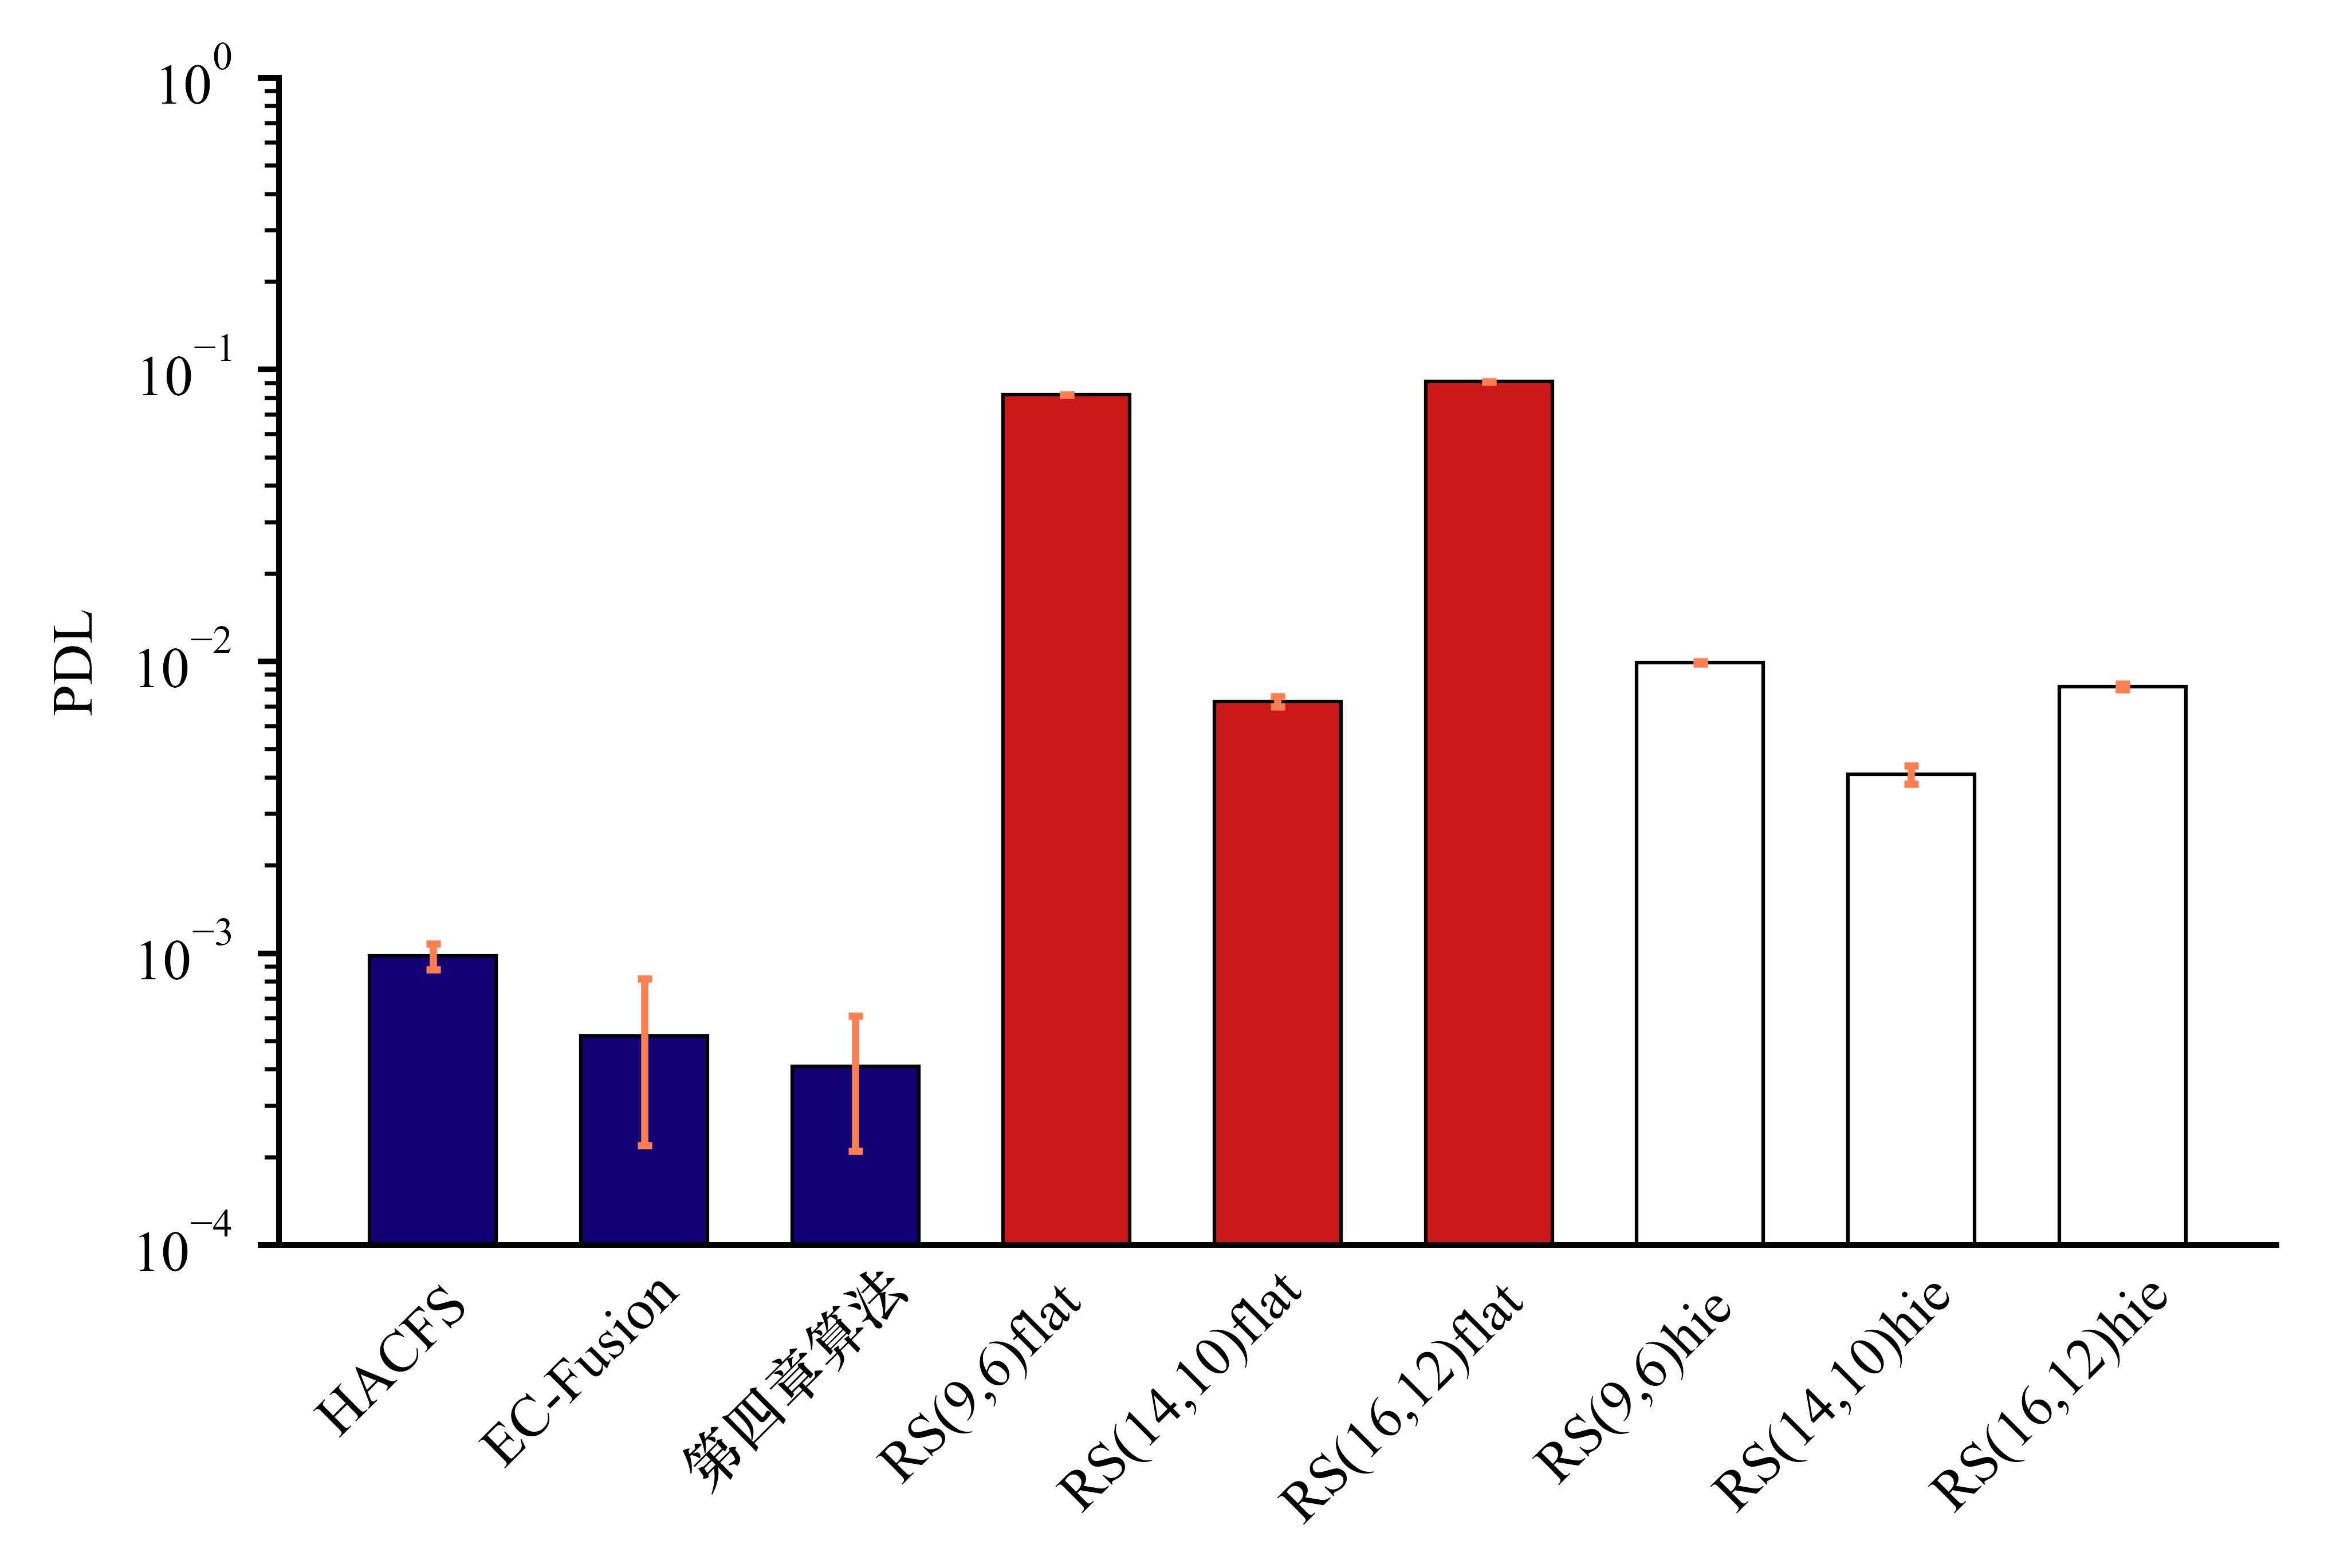
\includegraphics [scale=0.06]{figures/5-4.jpg}
	\caption{原型系统的PDL实验结果}
	\label{fig:5-4}
\end{figure}

\subsection{NOMDL参数实验结果}
如图~\ref{fig:5-5}所示是NOMDL多次实验的结果,误差区间是$\pm 2.5\%$。
与PDL测试结果相同的是,对于$y$轴同样进行了对数化处理,
依然可以看出平均水平而言,层次放置的RS码依然比水平放置的RS码的NOMDL指数更低,
也就意味着数据丢失量(以字节为单位)与存储容量的比例更低,
整个系统的数据存储的可用数据比例更高,此外三种混合纠删码策略也比层次放置的单一纠删码的性能要更好,
且LRC\&HH方案比其他两种方案要更好,因为其本身利用了不同编码族的特性并进行了相应的切换算法的优化,并且得益于
重建修复调度的优化,
NOMDL平均
降低了40\%$\sim$42.5\%。 


\begin{figure}[htbp]
	\centering
	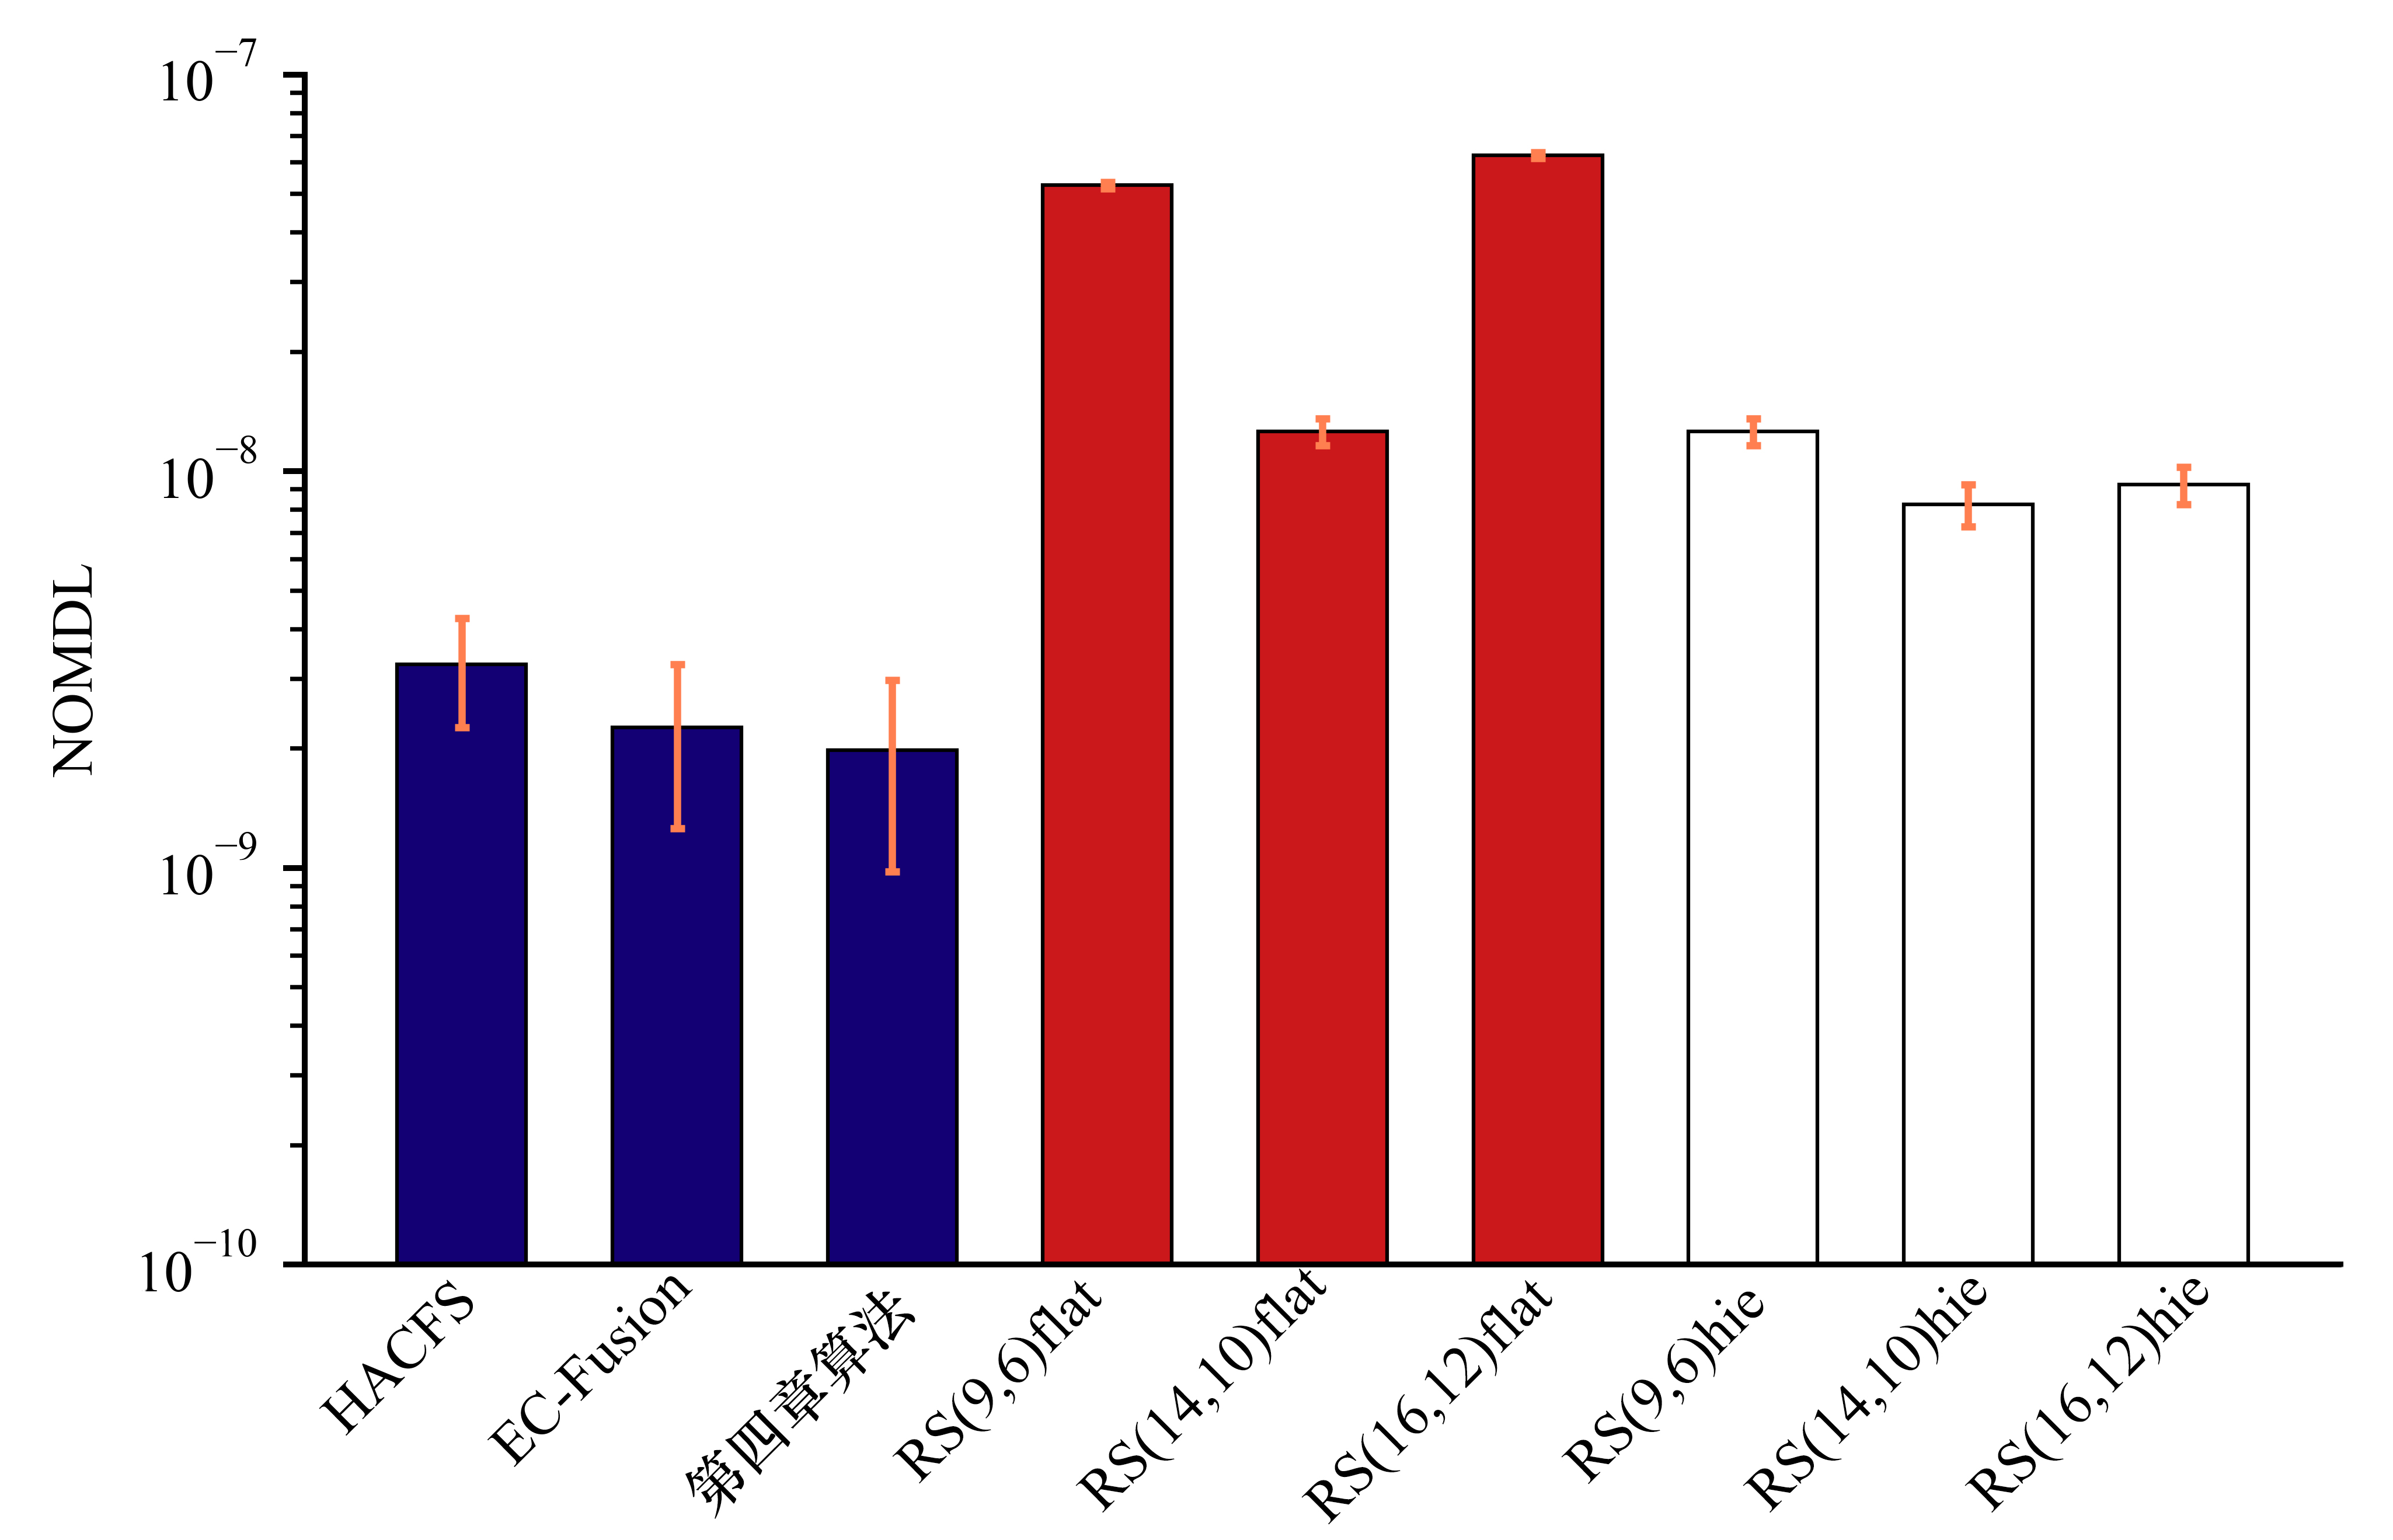
\includegraphics [scale=0.06]{figures/5-5.jpg}
	\caption{原型系统的NOMDL实验结果}
	\label{fig:5-5}
\end{figure}

\subsection{BR参数实验结果}

如图~\ref{fig:5-6}所示是BR多次实验的结果,误差区间是$\pm 1.7\%$。 
就平均水平而言,层次放置的RS码依然比水平放置的RS码的BR指数更低,
也就意味着存储一个数据块的子系统由于短暂的或永久的故障而不能直接访问该块的时间的比例大大减少,
整个系统数据存储的可访问时间占据全运行时间的比例更高。
RS$(16,12)$的冗余性能非常优越,得益于其有着更多的编码块冗余和在层次放置策略下更加
低的跨机柜之间的数据传输量,此外三种混合纠删码策略也比层次放置的单一纠删码的性能要更好,
且LRC\&HH方案和EC-Fuison在BR指数上基本持平,说明两种编码方案的在系统的访问时间上的可靠性是相近的,
BR平均降低了35.6\%$\sim$37.8\%。

\begin{figure}[htbp]
	\centering
	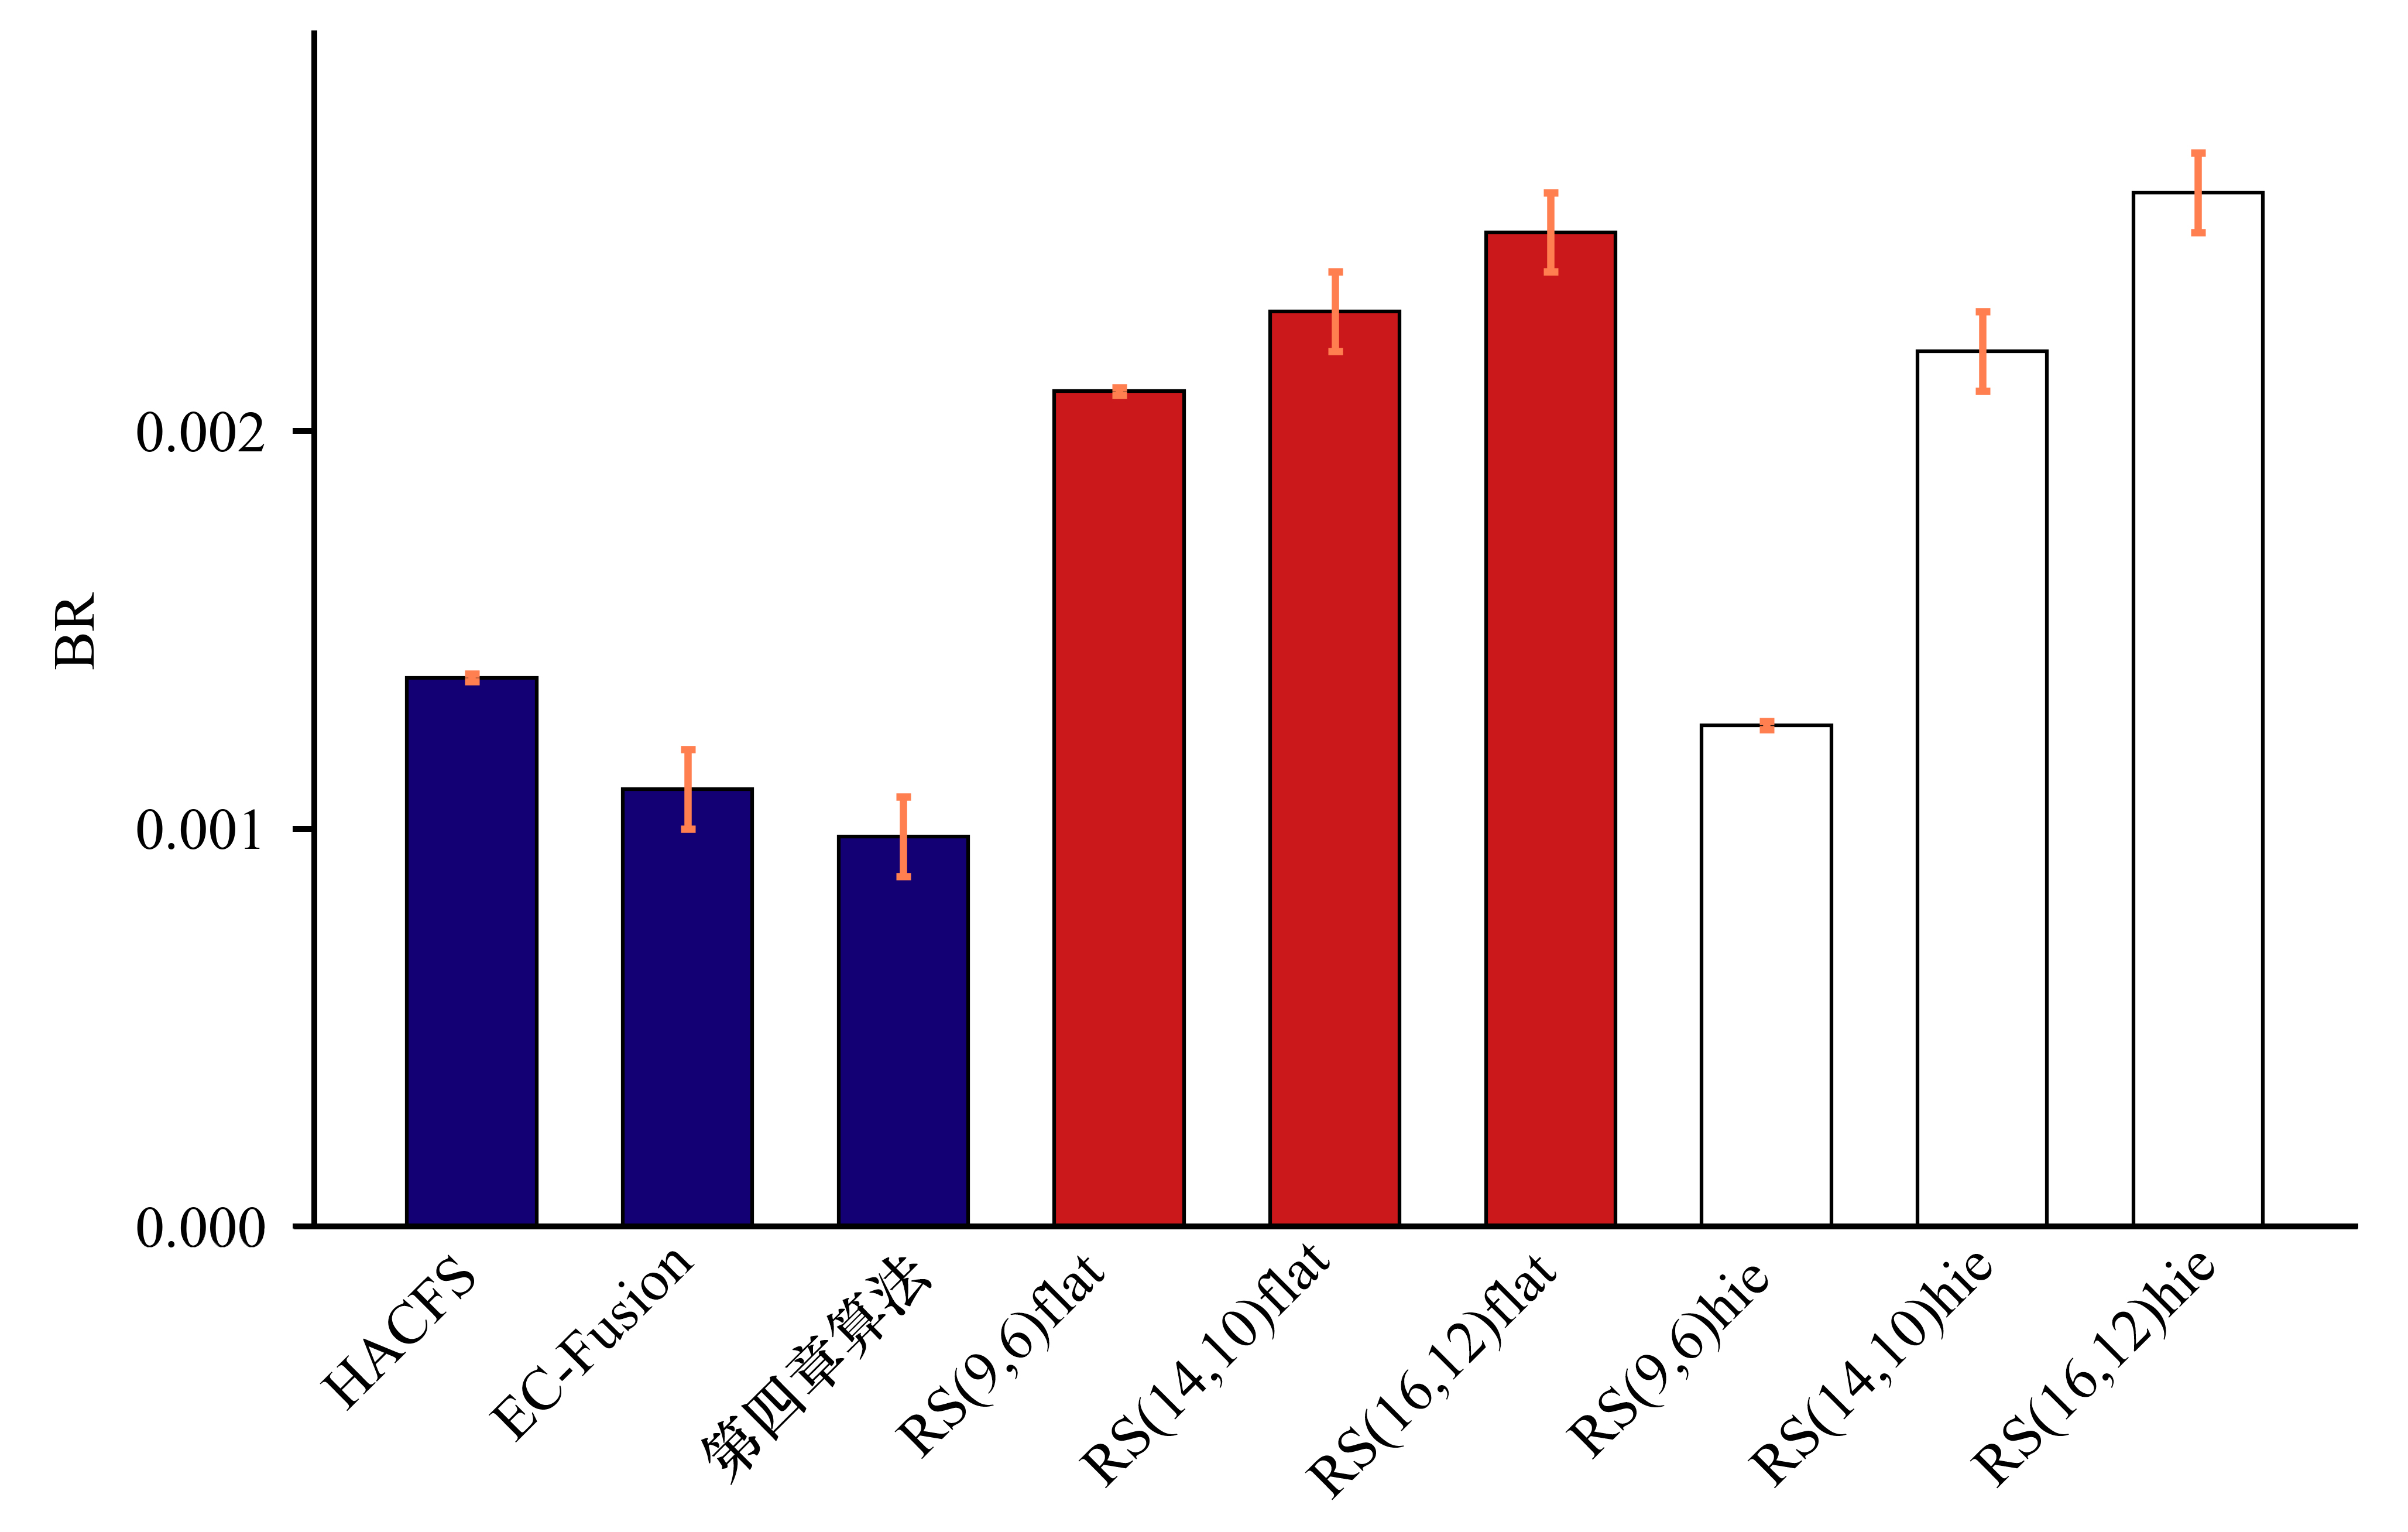
\includegraphics [scale=0.06]{figures/5-6.jpg}
	\caption{原型系统的BR实验结果}
	\label{fig:5-6}
\end{figure}



\section{本章小结}
在前两章的基础上,本章为了验证预先修复技术和混合纠删码修复技术在实际应用中的性能,设计
并实现了一个容错存储原型系统。容错存储原型系统设计主要包含以下模块:存储中心架构,节点故障模型,混合
纠删码策略,节点放置策略,可靠性度量指标,事件处理模式。实验结果表明,基于混合纠删码结构的容错存储原型系统具有较高的可靠性,
PDL参数平均降低了30\%$\sim$35\%,NOMDL平均
降低了40\%$\sim$42.5\%,BR平均降低了35.6\%$\sim$37.8\%。

